% Options for packages loaded elsewhere
\PassOptionsToPackage{unicode}{hyperref}
\PassOptionsToPackage{hyphens}{url}
\PassOptionsToPackage{space}{xeCJK}
%
\documentclass[
  nottoc]{article}

\usepackage{amsmath,amssymb}
\usepackage{iftex}
\ifPDFTeX
  \usepackage[T1]{fontenc}
  \usepackage[utf8]{inputenc}
  \usepackage{textcomp} % provide euro and other symbols
\else % if luatex or xetex
  \usepackage{unicode-math}
  \defaultfontfeatures{Scale=MatchLowercase}
  \defaultfontfeatures[\rmfamily]{Ligatures=TeX,Scale=1}
\fi
\usepackage{lmodern}
\ifPDFTeX\else  
    % xetex/luatex font selection
    \setmainfont[]{Crimson}
  \ifXeTeX
    \usepackage{xeCJK}
    \setCJKmainfont[]{Noto Serif KR}
          \fi
  \ifLuaTeX
    \usepackage[]{luatexja-fontspec}
    \setmainjfont[]{Noto Serif KR}
  \fi
\fi
% Use upquote if available, for straight quotes in verbatim environments
\IfFileExists{upquote.sty}{\usepackage{upquote}}{}
\IfFileExists{microtype.sty}{% use microtype if available
  \usepackage[]{microtype}
  \UseMicrotypeSet[protrusion]{basicmath} % disable protrusion for tt fonts
}{}
\makeatletter
\@ifundefined{KOMAClassName}{% if non-KOMA class
  \IfFileExists{parskip.sty}{%
    \usepackage{parskip}
  }{% else
    \setlength{\parindent}{0pt}
    \setlength{\parskip}{6pt plus 2pt minus 1pt}}
}{% if KOMA class
  \KOMAoptions{parskip=half}}
\makeatother
\usepackage{xcolor}
\usepackage[left=1in,right=1in,marginparwidth=1.5in,twoside=true]{geometry}
\setlength{\emergencystretch}{3em} % prevent overfull lines
\setcounter{secnumdepth}{3}
% Make \paragraph and \subparagraph free-standing
\makeatletter
\ifx\paragraph\undefined\else
  \let\oldparagraph\paragraph
  \renewcommand{\paragraph}{
    \@ifstar
      \xxxParagraphStar
      \xxxParagraphNoStar
  }
  \newcommand{\xxxParagraphStar}[1]{\oldparagraph*{#1}\mbox{}}
  \newcommand{\xxxParagraphNoStar}[1]{\oldparagraph{#1}\mbox{}}
\fi
\ifx\subparagraph\undefined\else
  \let\oldsubparagraph\subparagraph
  \renewcommand{\subparagraph}{
    \@ifstar
      \xxxSubParagraphStar
      \xxxSubParagraphNoStar
  }
  \newcommand{\xxxSubParagraphStar}[1]{\oldsubparagraph*{#1}\mbox{}}
  \newcommand{\xxxSubParagraphNoStar}[1]{\oldsubparagraph{#1}\mbox{}}
\fi
\makeatother


\providecommand{\tightlist}{%
  \setlength{\itemsep}{0pt}\setlength{\parskip}{0pt}}\usepackage{longtable,booktabs,array}
\usepackage{calc} % for calculating minipage widths
% Correct order of tables after \paragraph or \subparagraph
\usepackage{etoolbox}
\makeatletter
\patchcmd\longtable{\par}{\if@noskipsec\mbox{}\fi\par}{}{}
\makeatother
% Allow footnotes in longtable head/foot
\IfFileExists{footnotehyper.sty}{\usepackage{footnotehyper}}{\usepackage{footnote}}
\makesavenoteenv{longtable}
\usepackage{graphicx}
\makeatletter
\def\maxwidth{\ifdim\Gin@nat@width>\linewidth\linewidth\else\Gin@nat@width\fi}
\def\maxheight{\ifdim\Gin@nat@height>\textheight\textheight\else\Gin@nat@height\fi}
\makeatother
% Scale images if necessary, so that they will not overflow the page
% margins by default, and it is still possible to overwrite the defaults
% using explicit options in \includegraphics[width, height, ...]{}
\setkeys{Gin}{width=\maxwidth,height=\maxheight,keepaspectratio}
% Set default figure placement to htbp
\makeatletter
\def\fps@figure{htbp}
\makeatother
% definitions for citeproc citations
\NewDocumentCommand\citeproctext{}{}
\NewDocumentCommand\citeproc{mm}{%
  \begingroup\def\citeproctext{#2}\cite{#1}\endgroup}
\makeatletter
 % allow citations to break across lines
 \let\@cite@ofmt\@firstofone
 % avoid brackets around text for \cite:
 \def\@biblabel#1{}
 \def\@cite#1#2{{#1\if@tempswa , #2\fi}}
\makeatother
\newlength{\cslhangindent}
\setlength{\cslhangindent}{1.5em}
\newlength{\csllabelwidth}
\setlength{\csllabelwidth}{3em}
\newenvironment{CSLReferences}[2] % #1 hanging-indent, #2 entry-spacing
 {\begin{list}{}{%
  \setlength{\itemindent}{0pt}
  \setlength{\leftmargin}{0pt}
  \setlength{\parsep}{0pt}
  % turn on hanging indent if param 1 is 1
  \ifodd #1
   \setlength{\leftmargin}{\cslhangindent}
   \setlength{\itemindent}{-1\cslhangindent}
  \fi
  % set entry spacing
  \setlength{\itemsep}{#2\baselineskip}}}
 {\end{list}}
\usepackage{calc}
\newcommand{\CSLBlock}[1]{\hfill\break\parbox[t]{\linewidth}{\strut\ignorespaces#1\strut}}
\newcommand{\CSLLeftMargin}[1]{\parbox[t]{\csllabelwidth}{\strut#1\strut}}
\newcommand{\CSLRightInline}[1]{\parbox[t]{\linewidth - \csllabelwidth}{\strut#1\strut}}
\newcommand{\CSLIndent}[1]{\hspace{\cslhangindent}#1}

\makeatletter
\@ifpackageloaded{caption}{}{\usepackage{caption}}
\AtBeginDocument{%
\ifdefined\contentsname
  \renewcommand*\contentsname{Table of contents}
\else
  \newcommand\contentsname{Table of contents}
\fi
\ifdefined\listfigurename
  \renewcommand*\listfigurename{List of Figures}
\else
  \newcommand\listfigurename{List of Figures}
\fi
\ifdefined\listtablename
  \renewcommand*\listtablename{List of Tables}
\else
  \newcommand\listtablename{List of Tables}
\fi
\ifdefined\figurename
  \renewcommand*\figurename{Figure}
\else
  \newcommand\figurename{Figure}
\fi
\ifdefined\tablename
  \renewcommand*\tablename{Table}
\else
  \newcommand\tablename{Table}
\fi
}
\@ifpackageloaded{float}{}{\usepackage{float}}
\floatstyle{ruled}
\@ifundefined{c@chapter}{\newfloat{codelisting}{h}{lop}}{\newfloat{codelisting}{h}{lop}[chapter]}
\floatname{codelisting}{Listing}
\newcommand*\listoflistings{\listof{codelisting}{List of Listings}}
\makeatother
\makeatletter
\makeatother
\makeatletter
\@ifpackageloaded{caption}{}{\usepackage{caption}}
\@ifpackageloaded{subcaption}{}{\usepackage{subcaption}}
\makeatother

\ifLuaTeX
  \usepackage{selnolig}  % disable illegal ligatures
\fi
\usepackage{bookmark}

\IfFileExists{xurl.sty}{\usepackage{xurl}}{} % add URL line breaks if available
\urlstyle{same} % disable monospaced font for URLs
\hypersetup{
  pdftitle={Emergent Abstract Ordering Preferences in Large Language Models},
  pdfauthor={Zachary Nicholas Houghton; Kenji Sagae; Emily Morgan},
  hidelinks,
  pdfcreator={LaTeX via pandoc}}


\title{Emergent Abstract Ordering Preferences in Large Language Models}
\author{Zachary Nicholas Houghton \and Kenji Sagae \and Emily Morgan}
\date{}

\begin{document}
\maketitle


\section{Introduction}\label{sec-introduction}

Large language models have stormed the media in the last few years and
become a popular topic in the scientific literature. Their historic rise
to fame has brought with them many heated debates regarding whether
large language models constitute human-like models of language or
whether what they are doing is completely different from humans
(\citeproc{ref-benderDangersStochasticParrots2021}{Bender et al., 2021};
\citeproc{ref-piantadosiChapterModernLanguage}{Piantadosi, 2023};
\citeproc{ref-piantadosiMeaningReferenceLarge2022}{Piantadosi \& Hill,
2022}).

Many of these debates have centered around the tradeoff between
computation and storage: how much are these models simply reproducing
from their training data vs how much of their productions are novel
utterances using learned linguistic patterns. On one hand, there is no
doubt that large language models store and reproduce large chunks of
language. In fact, OpenAI is even being sued by \emph{The New York
Times} for allegedly reproducing entire articles verbatim
(\citeproc{ref-nyt_v_openai}{\emph{{The New York Times Company v.
Microsoft Corporation, OpenAI, Inc., OpenAI LP, OpenAI GP, LLC, OpenAI,
LLC, OpenAI OpCo LLC, OpenAI Global LLC, OAI Corporation, LLC, and
OpenAI Holdings, LLC}}, 2024}). This sentiment -- that large language
models are nothing but glorified copy cats -- has been echoed by several
other prominent linguists
(\citeproc{ref-benderDangersStochasticParrots2021}{Bender et al., 2021};
\citeproc{ref-bender2020climbing}{Bender \& Koller, 2020}; c.f.,
\citeproc{ref-piantadosiChapterModernLanguage}{Piantadosi, 2023}).

Specifically, proponents of the ``LLMs as copy cats'' argument have
pointed out that large language models are trained on an inconceivably
large amount of data. For example, the OLMo models were trained on
trillions of tokens
(\citeproc{ref-groeneveldOLMoAcceleratingScience2024}{Groeneveld et al.,
2024})\footnote{This is magnitudes larger than the 350 million words
  that the average college-aged speaker has seen in their lifetime
  (\citeproc{ref-levy2012}{Levy et al., 2012}).}. As such, it is
extremely difficult to determine whether utterances produced by an LLM
are truly novel, or whether they are simply reproduced from their
training data. This is further complicated by the fact that training
data for LLMs is typically either not publicly available, or so huge
that it's incredibly difficult to work with. On the other hand, it is
clear that large language models are learning at least some linguistic
patterns. For example, McCoy et al. (\citeproc{ref-mccoy2023much}{2023})
demonstrated that Chat GPT-2 is able to generate well-formed novel words
as well as well-formed novel syntactic structures, however they found
that it still copies extensively.

A similar debate in the field has centered around whether large language
models learn any knowledge about the meaning of words. For example,
Bender \& Koller (\citeproc{ref-bender2020climbing}{2020}) have argued
that large language models, which are only trained on the form, have no
way of learning anything about meaning. They pointed out that large
language models do not have the rich information that humans receive,
such as the referent of the form. However, Piantadosi \& Hill
(\citeproc{ref-piantadosiMeaningReferenceLarge2022}{2022}) have
countered by arguing that co-occurrence statistics can be extremely
informative about a word's meaning. For example, they argued that many
words, such as ``justice'', contain no clear referent and instead have
to be learned by humans based on the context that they occur in. It
seems plausible that large language models could learn at least some
information about meanings similarly.

These debates, however, have been highly theoretical and speculative and
very few empirical studies have been done to actually investigate these
questions (\citeproc{ref-lasri2022subject}{Lasri et al., 2022}; c.f.,
\citeproc{ref-lebrun2022evaluating}{LeBrun et al., 2022};
\citeproc{ref-mccoy2023much}{McCoy et al., 2023}). Thus in the present
paper we address these debates by taking an in-depth look at large
language models' abilities to abstract across their training data.

Our specific contributions are as follows: We make a 3-grams corpus of
Dolma (\citeproc{ref-soldainiDolmaOpenCorpus2024}{Soldaini et al.,
2024}) along with the scripts to reproduce it open-access. We also use
this corpus to create novel binomials that the OLMo 7B model
(\citeproc{ref-groeneveldOLMoAcceleratingScience2024}{Groeneveld et al.,
2024}) has never seen and demonstrate that OLMo shows evidence of using
learned abstract ordering preferences. Finally, we demonstrate a
timescale of these preferences emerging over training that can be used
to generate predictions about human learning.

\subsection{Abstractions in Large Language
Models}\label{abstractions-in-large-language-models}

The evidence for learned abstractions in large language models is
extremely mixed. For example, Haley (\citeproc{ref-haley2020bert}{2020})
demonstrated that many of the BERT models are not able to reliably
determine the plurality of novel words. Specifically, they tasked BERT
with choosing between two forms of a novel noun: the plural form and the
singular form. They tested BERT on 5 different languages: English,
German, Dutch, Spanish, and French. Interestingly, they also had a
condition which contained a prime. In English, the prime sentence was:
``This is a \_\_\_\_\_'', with the singular form of the noun replacing
the blank space. Humans are able to use this contextual information to
determine the plural form of the noun reliably, and Haley
(\citeproc{ref-haley2020bert}{2020}) argued that it is theoretically
possible for BERT to learn to do so as well using self-attention. While
BERT was able to perform better-than-chance on novel nouns,
cross-linguistically it failed to use information about the prime
sentence to achieve better performance.

On the other hand, Lasri et al. (\citeproc{ref-lasri2022subject}{2022})
demonstrated that BERT can generalize well to novel subject-verb pairs.
Specifically, they tested BERT's performance on novel sentences along
with semantically incoherent but syntactically sensible sentences (e.g.,
\emph{colorless green ideas sleep furiously}). They found that BERT
performs well on items it wasn't trained on but struggles more on
semantically incoherent sentences than humans do. Similarly, as
mentioned earlier, McCoy et al. (\citeproc{ref-mccoy2023much}{2023})
examined to what extent GPT-2 was simply copying its training data vs
producing novel utterances. They found that while GPT-2 copies
extensively, it also produces both novel words as well as novel
syntactic structures.

Finally, there is evidence that transformer models can learn
abstractions from other domains as well. For example, Tartaglini et al.
(\citeproc{ref-tartaglini2023deep}{2023}) examined the ability of a
transformer model in a same-different task (i.e., determining if two
entities, e.g., two shapes, in an image are the same or different). They
found that certain models can reach near perfect accuracy on items they
have never seen before. They argued that this demonstrates their
abilities to learn abstract representations.

\subsection{Abstractions in Humans}\label{abstractions-in-humans}

Abstractions have been a part of just about every linguistic theory out
there, including both generativist and non-generativist theories. This
is for good reason, too: one of the hallmarks of human language learning
is the ability to produce novel, never-heard-before utterances. In order
to do so, most theories posit that humans leverage their remarkable
ability to learn linguistic patterns beyond simple co-occurrence rates
(c.f., \citeproc{ref-ambridge2020}{Ambridge, 2020}). For example, when
presented a novel noun, children are able to consistently produce the
proper plural form of that noun (\citeproc{ref-berko}{Berko, 1958}).
Similarly, children are able to abstract across different contexts to
learn a word's general meaning (\citeproc{ref-yu2007rapid}{Yu \& Smith,
2007}).

Abstractions are useful because when humans produce a novel utterance
that they have never heard before, their novel utterances contain a
level of systematicity that allows the interlocutor to understand it
with very little difficulty. This is even the case for binomials (e.g.,
\emph{cat and dog}), whose order does not particularly affect the
meaning of the utterance. Binomial ordering preferences are
well-documented in the literature. For example, Morgan \& Levy
(\citeproc{ref-morganAbstractKnowledgeDirect2016}{2016}) demonstrated
that humans show ordering preferences for binomials beyond simply
preferring the more frequent ordering (e.g., preferring male-coded words
before female-coded words). They coded a list of binomials for a variety
of semantic constraints, phonological constraints, and metric
constraints that affect human ordering preferences for binomials
(\citeproc{ref-benorChickenEggProbabilistic2006}{Benor \& Levy, 2006}).
They found that human ordering preferences were driven by abstract
ordering preferences, such as a preference to place short words before
longer words, even after accounting for the relative frequency (the
proportion of each ordering that a binomial occurs in corpus data). In
other words, human ordering preferences are driven by both the observed
preferences in corpus data (i.e., the number of times they've
encountered each ordering of the binomial) as well as by abstract
ordering preferences
(\citeproc{ref-morganAbstractKnowledgeDirect2016}{Morgan \& Levy,
2016}). Specifically, they developed a model to quantify the abstract
ordering preferences of humans for a given binomial in English. The
model predicts the probability that a binomial expression is realized as
\emph{A and B} (the alphabetical form was used as a neutral reference
order) as a function of constraints that have been shown to influence
binomial ordering preferences in humans (e.g.~a preference to place more
culturally-central words first,
\citeproc{ref-benorChickenEggProbabilistic2006}{Benor \& Levy, 2006}).

Morgan \& Levy (\citeproc{ref-morganAbstractKnowledgeDirect2016}{2016})
demonstrated that the model's predicted abstract ordering preferences
are not the same as the observed preferences in corpus data (i.e., the
model wasn't simply predicting the more frequent ordering). Despite
this, however, they showed in both a forced-choice task and a self-paced
reading task that abstract ordering preferences drive, to some extent,
both novel and attested binomial orderings. In other words, the ordering
preference for a specific binomial cannot be predicted purely from the
proportion of occurrences in the alphabetical order to the occurrences
in nonalphabetical. This suggests that humans are not simply reproducing
their input, but learning abstract ordering preferences from the data.

\subsection{Present Study}\label{present-study}

In the present study we examine whether large language models are simply
copying their input, or whether they are learning more abstract
linguistics patterns. We use binomials as a test case because human
ordering preferences deviate from the observed preferences for them
(that is, humans don't simply prefer the more frequent ordering).
Further, we use novel binomials that OLMo has never seen before.
Therefore any preference the model has cannot be driven by experience
with the specific item.

Specifically, in Experiment 1 we examine whether OLMo's 7B model
(\citeproc{ref-groeneveldOLMoAcceleratingScience2024}{Groeneveld et al.,
2024}) is sensitive to abstract ordering preferences for novel binomials
that the model has never seen before. We also examine the individual
constraints that drive abstract ordering preferences in humans, such as
the preference for short words before long words, to determine whether
OLMo is sensitive to the same constraints in the same way as humans. In
Experiment 2, we examine the same questions at different stages of the
model's learning in order to determine how these abstract ordering
preferences emerge as a function of the training.

\section{Dataset}\label{dataset}

\subsection{Dolma}\label{dolma}

For both experiments, we use the dataset described in this section. In
order to examine whether large language models learn preferences above
and beyond simply memorizing co-occurrence rates, we created a 3-grams
corpus of Dolma (\citeproc{ref-soldainiDolmaOpenCorpus2024}{Soldaini et
al., 2024}). Specifically, we used Dolma version 1\_7 (2.05 trillion
tokens), which was used to train OLMo-7B-v1.7
(\citeproc{ref-groeneveldOLMoAcceleratingScience2024}{Groeneveld et al.,
2024}). Our corpus contains every 3-gram (ignoring punctuation and
capitalization) in the Dolma corpus, as well as the number of times that
3-gram appeared. Similarly, in order to calculate individual
word-frequencies we also created a 1-gram corpus of Dolma.

We then created a list of binomials and searched the corpus to find a
list of binomials that did not occur in the Dolma corpus. We eliminated
binomials which occurred more than zero times in either their
alphabetical or nonalphabetical orderings. Thus, OLMo has had no
experience with either ordering of any of our binomials. Individual word
frequencies were also calculated for these items using the 1-grams
corpus of Dolma. Our full list of items is presented in full in the
appendix section\footnote{Our code for the corpus and the analyses run
  in this paper can also be found at:
  \url{github.com/\%5Banonymous\%5D}.} (Section
Section~\ref{sec-full-list-of-stimuli}).

\subsection{Abstract Ordering Preferences
Corpus}\label{abstract-ordering-preferences-corpus}

In order to examine whether large language models are learning
preferences similar to humans, we calculated the abstract ordering
preference value for each of our binomials (following
\citeproc{ref-morganAbstractKnowledgeDirect2016}{Morgan \& Levy, 2016}).
Morgan \& Levy (\citeproc{ref-morganAbstractKnowledgeDirect2016}{2016})
demonstrated that their model's estimated abstract ordering preference
value is a significant predictor of human binomial ordering preferences,
even after accounting for the frequency of the binomial. Abstract
ordering preferences are calculated from a mix of semantic and
phonological properties that human binomial ordering preferences have
been shown to be sensitive to
(\citeproc{ref-benorChickenEggProbabilistic2006}{Benor \& Levy, 2006}).
For each of these constraints, a positive value indicates a preference
for the alphabeticaly first word to be placed first (a neutral reference
order). A negative value indicates a preference for the nonalphabetical
word to be placed first. For example, a positive value of \emph{Freq}
indicates that the alphabetical word is more frequent and thus is
predicted to be placed first, while a negative value indicates that the
nonalphabetical word is more frequent. The constraints are as follows:

\begin{itemize}
\item
  \textbf{Formal Markedness}: The word with more general meaning or
  broader distribution comes first. For example, in \emph{boards and
  two-by-fours}, boards are a broader class of which two-by-fours is one
  member.
\item
  \textbf{Perceptual Markedness}: Elements that are more closely
  connected to the speaker come first. This constraint encompasses
  Cooper \& Ross (\citeproc{ref-cooper1975world}{1975})`s (1975) `Me
  First' constraint and includes numerous subconstraints, e.g.: animates
  precede inanimates; concrete words precede abstract words. For
  example, in \emph{deer and trees}, deer are animate while trees are
  inanimate.
\item
  \textbf{Cultural Centrality}: More culturally central or common
  elements appear first. For example, in \emph{see and hear} seeing is
  the more salient form of perception.
\item
  \textbf{Power}: The more powerful or culturally prioritized word comes
  first. For example, in \emph{clergymen and parishioners}, clergymen
  have higher rank within the church.
\item
  \textbf{Intensity}: Elements with more intensity appear first.
\item
  \textbf{Iconicity}: When two elements are sequential they should
  appear in the appropriate sequence.
\item
  \textbf{Frequency}: The more frequent element should appear first.
\item
  \textbf{Length}: The shorter word should appear first.
\item
  \textbf{Lapse:} The ordering that avoids multiple unstressed syllables
  is preferred.
\item
  \textbf{Final Stress}: The ordering that avoids the final syllable of
  the second word being stressed is preferred.
\end{itemize}

\section{Experiment 1}\label{experiment-1}

In Experiment 1, we examine whether OLMo-7B's ordering preferences are
driven by abstract ordering preferences for novel binomials. In order to
do so, we obtain ordering preferences for each of the binomials in our
dataset which have been coded for the abstract ordering preference
constraints from Morgan \& Levy
(\citeproc{ref-morganAbstractKnowledgeDirect2016}{2016}). If OLMo has
developed any abstract ordering preferences, it should show prefer some
orderings over others. If it is just reproducing the binomials in
ordering based purely off the frequency of the items in its input, we
should see only an effect of frequency (i.e., it should simply place the
more frequent word first).

\subsection{Methods}\label{methods}

\subsubsection{Language Model
Predictions}\label{language-model-predictions}

For each model, we calculated the ordering preferences of the
alphabetical form (a neutral reference point) for each binomial in the
dataset. The predicted probability of the alphabetical form was
calculated as the product of the model's predicted probability of each
word in the binomial. In order to accurately calculate the probability
of the first word in the binomial, each binomial was given the prefix
``Next item:''. Thus the probability of the alphabetical form, \emph{A
and B,} is:

\begin{equation}\phantomsection\label{eq-probalpha}{
\begin{aligned}
    P_{alphabetical} & = P(A|\text{`Next item:'} )\\      
    & \times P(and|\text{`Next item: A'})\\      
    & \times P(B|\text{`Next item: A and'})
\end{aligned}
}\end{equation}

\noindent where \emph{A} is the alphabetically first word in the
binomial and \emph{B} is the other word. Similarly, the probability of
the nonalphabetical form, \emph{B and A}, is:

\begin{equation}\phantomsection\label{eq-probnonalpha}{
\begin{aligned}    
P_{nonalphabetical} & = P(B|\text{`Next item:'})\\
& \times P(and|\text{`Next item: B'})\\
& \times P(A|\text{`Next item: B and'})
\end{aligned}
}\end{equation}

Finally, we calculated the log odds ratio of the probability of the
alphabetical form to the probability of the nonalphabetical form to
obtain a single numeric value representing the overall ordering
preference for a given binomial. A larger positive value represents a
preference for the alphabetical form and a larger negative value
represents a preference for the nonalphabetical form:

\[
LogOdds(AandB) = log(\frac{P_{alphabetical}}{P_{nonalphabetical}})
\]

\subsubsection{Analyses}\label{analyses}

We present two mixed-effects analyses using Bayesian linear regression
models, implemented in \emph{brms} (\citeproc{ref-brms}{Bürkner, 2017})
with weak, uninformative priors. For each of our models, the intercept
represents the grand mean and the coefficient estimates represent the
distance from the grand mean. Bayesian statistics don't force us into a
binary interpretation of significance or non-significance, however we
can consider an estimate to be statistically significant if the credible
interval for that estimate excludes zero.

For both analyses, the dependent variable is \(LogOdds(AandB)\), which
was described above. Our dependent variable in the first analysis is the
abstract ordering preference for each binomial (\(AbsPref\))\footnote{We
  also ran a model examining whether the ordering preferences were
  driven by the bigram probabilities of the trigram, however bigram
  probabilities turned out not to be a good predictor of ordering
  preferences.}. Our dependent variables in the second analysis are the
individual constraints that are used to calculate \(AbsPref\). The model
equations are below in Equation~\ref{eq-m1} and Equation~\ref{eq-m2}.
Note that Formal Markedness and Iconicity were dropped from the second
model because the constraint values were zero for all of the binomials.
Further, our constraints demonstrated a level of co-linearity.
Co-linearity can result in poor model estimates and inflated credible
intervals. In order to deal with this, we dropped the constraint with
the highest variance inflation factor (which turned out to be the lapse
constraint). We then performed backward model selection and dropped the
predictors whose credible intervals were most centered around zero. This
resulted in dropping the no final stress, intense, and percept
constraints. We acknowledge that this approach is quite exploratory and
thus interpretations at the level of the individual constraint must be
taken with a grain of salt.

\begin{equation}\phantomsection\label{eq-m1}{
LogOdds(AandB) \sim AbsPref
}\end{equation}

\begin{equation}\phantomsection\label{eq-m2}{
LogOdds(AandB) \sim Culture + Power + Freq + Len + Lapse + FinalStress
}\end{equation}

\subsection{Results}\label{results}

The results for the first analysis are presented below in
Table~\ref{tbl-exp1m1}. Our results suggest that there is a main-effect
of abstract ordering preference for OLMo's 7B model. A visualization of
these results can be found below in Figure~\ref{fig-exp1m1}.

\begin{longtable}[]{@{}lllll@{}}

\toprule\noalign{}
& Estimate & Est.Error & Q2.5 & Q97.5 \\
\midrule\noalign{}
\endhead
\bottomrule\noalign{}
\endlastfoot
Intercept & -1.370 & 0.636 & -2.672 & -0.222 \\
AbsPref & 2.547 & 1.274 & 0.291 & 5.151 \\


\caption{\label{tbl-exp1m1}Model results examining the effect of AbsPref
on LogOdds(AandB).}

\tabularnewline
\end{longtable}

\begin{figure}

\centering{

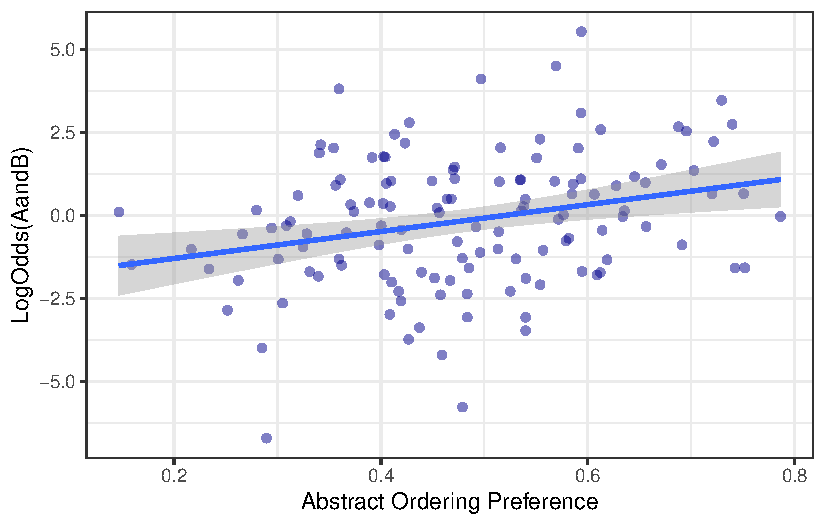
\includegraphics[width=0.8\textwidth,height=\textheight]{nonce_binoms_writeup_files/figure-pdf/fig-exp1m1-1.pdf}

}

\caption{\label{fig-exp1m1}Visualization of the effects of AbsPref on
LogOdds(AandB)}

\end{figure}%

While these results suggest that the large language models' ordering
preferences are sensitive to similar factors as humans, it's unclear
whether this similarity holds on the level of the individual
constraints. Thus, in the second analysis we examine which specific
constraints the model is sensitive to, and to what extent. For this
analysis, following Houghton et al.
(\citeproc{ref-houghtonTaskdependentConsequencesDisfluency2024}{2024}),
we also present the percentage of posterior samples greater than zero.
The results of this analysis can be found below in
Table~\ref{tbl-exp1m2}. Further, a visualization can be found below in
Figure~\ref{fig-exp1m2}.

\begin{longtable}[]{@{}lllllr@{}}

\toprule\noalign{}
& Estimate & Est.Error & Q2.5 & Q97.5 & \% Samples \textgreater{} 0 \\
\midrule\noalign{}
\endhead
\bottomrule\noalign{}
\endlastfoot
Intercept & -0.132 & 0.163 & -0.451 & 0.185 & 20.750 \\
Culture & 0.414 & 0.254 & -0.078 & 0.916 & 94.945 \\
Power & 0.720 & 0.263 & 0.204 & 1.236 & 99.665 \\
Freq & 0.091 & 0.087 & -0.079 & 0.263 & 85.170 \\
Len & -0.209 & 0.134 & -0.476 & 0.052 & 5.870 \\


\caption{\label{tbl-exp1m2}Model results examining the effect of each
individual constraint on LogOdds(AandB).}

\tabularnewline
\end{longtable}

Perhaps surprisingly, the model is most sensitive to the Power
constraint (\(\beta\) = 0.723, CI-2.5 = 0.293, CI-97.5 = 0.155) ,
however there appears to be a weak effect of Culture as well, since 89\%
of the posterior samples are greater than zero despite the credible
interval crossing zero (\(\beta\) = 0.341, CI-2.5 = 0.276, CI-97.5 =
-0.198). Surprisingly, there also appears to be a negative effect of
length (\(\beta\) = -0.204, CI-2.5 = -0.502, CI-97.5 = 0.098), with a
slight preference to place the longer word first, which is the opposite
direction from what we see in humans.

\begin{figure}

\centering{

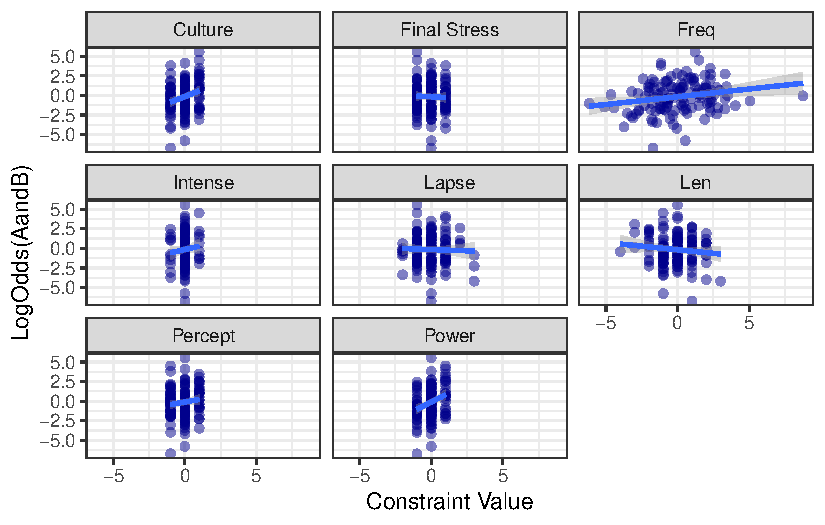
\includegraphics[width=0.8\textwidth,height=\textheight]{nonce_binoms_writeup_files/figure-pdf/fig-exp1m2-1.pdf}

}

\caption{\label{fig-exp1m2}Visualization of the effects of each
individual constraint on LogOdds(AandB).}

\end{figure}%

\subsection{Discussion}\label{discussion}

The present experiment found that OLMo-7B has learned abstract ordering
preferences even for novel binomials that it has never seen before.
Further, these ordering preferences aren't simply based on the
individual word frequencies. Specifically, we find a main-effect of
abstract ordering preferences on the model's binomial ordering
preferences. Additionally, we find a strong preference to place the more
powerful word first, a weak preference to place the more culturally
central word first, and a weak preference to place the longer word
first.

These results together suggest that the model is learning abstract
ordering preferences but these are not identical to humans. For example,
while humans also show a preference for placing the more powerful and
more culturally central words first, humans also prefer to place the
\emph{shorter} word first
(\citeproc{ref-morganModelingIdiosyncraticPreferences2015}{Morgan \&
Levy, 2015}, \citeproc{ref-morganAbstractKnowledgeDirect2016}{2016}).
However, we find the opposite finding: large language models prefer to
place the longer word first. One explanation for this is a difference in
terms of the input between humans and large language models. The length
constraint is determined by the number of syllables. Syllables are
salient cues in the audio that humans receive during learning
{[}\textbf{NEED CITATION{]}}, but it's less clear how salient of a cue
this is for large language models, who receive sub-word tokens (which
vary in their size, from being individual orthographic symbols to being
entire words\footnote{For example, both \emph{ictionary} and
  \emph{region} are individual tokens in OpenAI's models
  (\url{https://gist.github.com/s-macke/ae83f6afb89794350f8d9a1ad8a09193}).}).

\section{Experiment 2}\label{experiment-2}

In Experiment 1 we demonstrated that large language models are not
simply copying their training, but are learning some abstract ordering
preferences from their input. However, OLMo makes public various
checkpoints during the model's training, thus allowing us the
opportunity to examine how these preferences arise as a function of the
training. Thus, in Experiment 2 we examine the evolution of these
learned abstract ordering preferences as the model learns over time.

\subsection{Methods}\label{methods-1}

\subsubsection{Language Model
Predictions}\label{language-model-predictions-1}

Our language model predictions in Experiment 2 were obtained using the
same procedure as in Experiment 1. However, instead of calculating these
metrics only for the main model, we calculated them at various
checkpoints. These checkpoints are listed below, in terms of the steps
as well as the number of billions of tokens the model had been trained
on at that checkpoint:

\begin{itemize}
\item
  Step 0, 0B Tokens
\item
  Step 1000, 2B Tokens
\item
  Step 10000, 41B Tokens
\item
  Step 50000, 209B Tokens
\item
  Step 100000, 419B Tokens
\item
  Step 200000, 838B Tokens
\item
  Step 400000, Tokens 1677B
\end{itemize}

\subsubsection{Analysis}\label{analysis}

We ran the same two analyses as in Experiment 1, however, we ran these
analyses for the each of the checkpoints listed above.

\subsection{Results}\label{results-1}

Our model estimates for the effect of GenPref on LogOdds(AandB) at each
checkpoint are presented below in Table~\ref{tbl-exp2m1} and visualized
in Figure~\ref{fig-exp2m1}.

\begin{longtable}[]{@{}lllll@{}}

\toprule\noalign{}
Number of Tokens & Estimate & Est.Error & Q2.5 & Q97.5 \\
\midrule\noalign{}
\endhead
\bottomrule\noalign{}
\endlastfoot
0B & 0.189 & 0.789 & -1.303 & 1.787 \\
2B & 1.210 & 1.346 & -0.944 & 4.404 \\
41B & 0.869 & 1.167 & -1.119 & 3.472 \\
209B & 1.051 & 1.040 & -0.776 & 3.375 \\
419B & 1.700 & 1.216 & -0.355 & 4.326 \\
838B & 1.770 & 1.267 & -0.320 & 4.585 \\
1677B & 3.858 & 1.516 & 0.948 & 6.825 \\


\caption{\label{tbl-exp2m1}Model results examining the effect of AbsPref
on LogOdds(AandB) for each checkpoint.}

\tabularnewline
\end{longtable}

The model results are visualized below in Figure~\ref{fig-exp2m1}.

\begin{figure}

\centering{

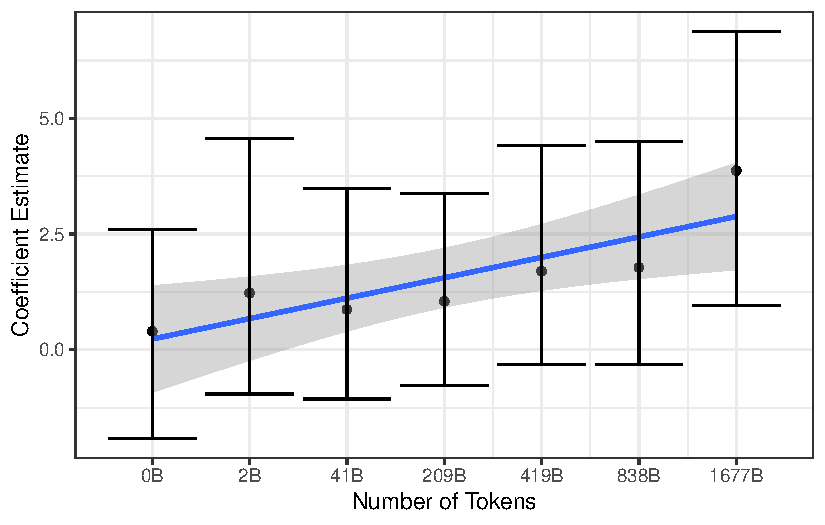
\includegraphics[width=0.7\textwidth,height=\textheight]{nonce_binoms_writeup_files/figure-pdf/fig-exp2m1-1.pdf}

}

\caption{\label{fig-exp2m1}Visualization of the model predictions for
the effect of AbsPref on LogOdds(AandB) for each checkpoint.}

\end{figure}%

Our results demonstrate that it takes quite a large number of tokens for
the model to learn the abstract ordering preferences. As
Figure~\ref{fig-exp2m1} demonstrates, the effect of abstract ordering
preference isn't convincing until the model has experienced 838 billion
tokens. However, it does appear that the model develops a slight
preference quite rapidly. For example, by 2 billion tokens there appears
to be a very slight (though unconvincing) effect of abstract ordering
preferences on the ordering of binomials.

Similar to Experiment 1, in our second analysis we present a breakdown
of the effects of each individual constraint. In this analysis, however,
we demonstrate the effect of each constraint at each checkpoint. The
full table results can be found in the
Section~\ref{sec-individual-constraints-at-each-checkpoint}, but we
present a visualization below in Figure~\ref{fig-exp2m2}.

\begin{figure}

\centering{

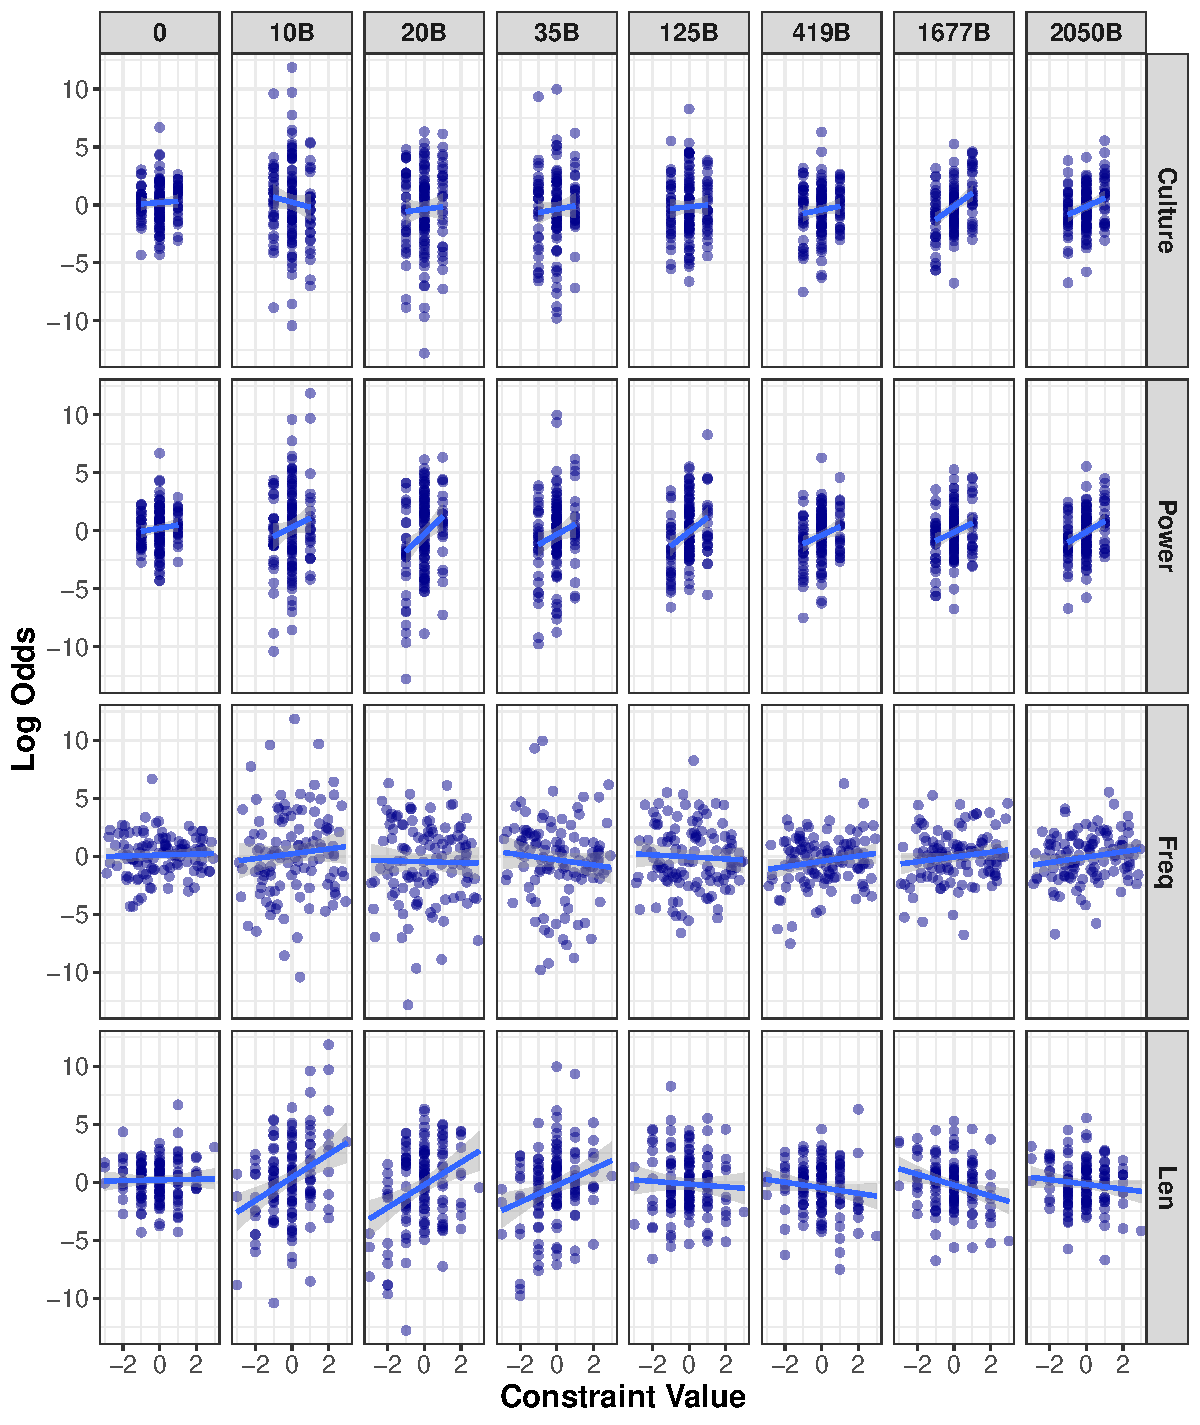
\includegraphics{nonce_binoms_writeup_files/figure-pdf/fig-exp2m2-1.pdf}

}

\caption{\label{fig-exp2m2}Visualization of the effect of each
constraint on the ordering preference at each checkpoint.}

\end{figure}%

Interestingly, it appears that early on the model already shows evidence
of learning human-like preferences. For example, by 10 billion tokens,
the model has learned to place more intense words first, shorter words
first, and more powerful words first. However, the model seems slower to
learn to place more culturally central words first. Further, as it
receives more training the effect of length undergoes a reversal in
direction.

\subsection{Discussion}\label{discussion-1}

Our results demonstrate that OLMo learns human-like ordering preferences
early on for most of the constraints, but takes longer to learn
human-like ordering preferences for the culture constraint. Further, the
model is human-like in its predictions for length early on, but as it
receives more training data it learns the opposite length prediction. It
is unclear what exactly is causing this reversal, but as we suggested
earlier it may be a function of the tokenization differences between
human input and large language models' input. We look forward to
examining this question in more depth in future studies.

Our results can also be interpreted as predictions for human data. For
example, it takes the model longer to learn the Culture constraint than
the other constraints. Is the same true for humans?

\section{Conclusion}\label{conclusion}

In the present study, we examined the ordering preferences in OLMo 7B's
main model as well as the model at various stages in learning. We found
that the main model shows human-like ordering preferences, with the
exception of a preference for longer words before shorter words.
Further, we show that while the effect of abstract ordering preference
on a whole takes a great deal of time (over 400 billion tokens to be
convincing), the model seems to pick up on individual constraints quite
early on, and initially even learns the correct direction of the length
constraint.

Our results suggest that large language models are not simply copying
their input, but are learning interesting, human-like phenomena from
their training. However, they are not learning identically to humans, as
demonstrated by the opposite direction of the length preference. This is
not surprising given the differences in tokenization methods.

\section{Limitations}\label{limitations}

The main limitation is the number of models tested. We only tested one
model in this study, so it's possible that other large language models
may demonstrate different ordering preferences. However, we believe that
the advantages of demonstrating an in-depth analysis of a single model
outweighs a more broad analysis of several models, especially given the
lack of easily available open access training data, which is crucial to
determining ordering preferences.

\clearpage

\section*{References}\label{references}
\addcontentsline{toc}{section}{References}

\phantomsection\label{refs}
\begin{CSLReferences}{1}{0}
\bibitem[\citeproctext]{ref-ambridge2020}
Ambridge, B. (2020). Against stored abstractions: A radical exemplar
model of language acquisition. \emph{First Language}, \emph{40}(5-6),
509--559. \url{https://doi.org/10.1177/0142723719869731}

\bibitem[\citeproctext]{ref-benderDangersStochasticParrots2021}
Bender, E. M., Gebru, T., McMillan-Major, A., \& Shmitchell, S. (2021).
\emph{FAccT '21: 2021 ACM Conference on Fairness, Accountability, and
Transparency}. 610--623. \url{https://doi.org/10.1145/3442188.3445922}

\bibitem[\citeproctext]{ref-bender2020climbing}
Bender, E. M., \& Koller, A. (2020). Climbing towards NLU: On meaning,
form, and understanding in the age of data. \emph{Proceedings of the
58th Annual Meeting of the Association for Computational Linguistics},
5185--5198.

\bibitem[\citeproctext]{ref-benorChickenEggProbabilistic2006}
Benor, S. B., \& Levy, R. (2006). The chicken or the egg? A
probabilistic analysis of english binomials. \emph{Language},
\emph{82}(2), 233--278. \url{https://doi.org/10.1353/lan.2006.0077}

\bibitem[\citeproctext]{ref-berko}
Berko, J. (1958). The Child's Learning of English Morphology.
\emph{{\emph{WORD}}}, \emph{14}(2-3), 150--177.
\url{https://doi.org/10.1080/00437956.1958.11659661}

\bibitem[\citeproctext]{ref-brms}
Bürkner, P.-C. (2017). Brms: An r package for bayesian multilevel models
using stan. \emph{Journal of Statistical Software}, \emph{80}, 128.
\url{https://www.jstatsoft.org/article/view/v080i01}

\bibitem[\citeproctext]{ref-cooper1975world}
Cooper, W. E., \& Ross, J. R. (1975). World order. \emph{Papers from the
Parasession on Functionalism}, \emph{11}, 63--111.

\bibitem[\citeproctext]{ref-groeneveldOLMoAcceleratingScience2024}
Groeneveld, D., Beltagy, I., Walsh, P., Bhagia, A., Kinney, R., Tafjord,
O., Jha, A. H., Ivison, H., Magnusson, I., Wang, Y., et al. (2024).
Olmo: Accelerating the science of language models. \emph{arXiv Preprint
arXiv:2402.00838}.

\bibitem[\citeproctext]{ref-haley2020bert}
Haley, C. (2020). This is a BERT. Now there are several of them. Can
they generalize to novel words? \emph{Proceedings of the Third
BlackboxNLP Workshop on Analyzing and Interpreting Neural Networks for
NLP}, 333--341.

\bibitem[\citeproctext]{ref-houghtonTaskdependentConsequencesDisfluency2024}
Houghton, Z., Kato, M., Baese-Berk, M., \& Vaughn, C. (2024).
Task-dependent consequences of disfluency in perception of native and
non-native speech. \emph{Applied Psycholinguistics}, 1--17.
\url{https://doi.org/10.1017/S0142716423000486}

\bibitem[\citeproctext]{ref-lasri2022subject}
Lasri, K., Seminck, O., Lenci, A., \& Poibeau, T. (2022). Subject verb
agreement error patterns in meaningless sentences: Humans vs. BERT.
\emph{arXiv Preprint arXiv:2209.10538}.

\bibitem[\citeproctext]{ref-lebrun2022evaluating}
LeBrun, B., Sordoni, A., \& O'Donnell, T. J. (2022). Evaluating
distributional distortion in neural language modeling. \emph{arXiv
Preprint arXiv:2203.12788}.

\bibitem[\citeproctext]{ref-levy2012}
Levy, R., Fedorenko, E., Breen, M., \& Gibson, E. (2012). The processing
of extraposed structures in english. \emph{Cognition}, \emph{122}(1),
12--36. \url{https://doi.org/10.1016/j.cognition.2011.07.012}

\bibitem[\citeproctext]{ref-mccoy2023much}
McCoy, R. T., Smolensky, P., Linzen, T., Gao, J., \& Celikyilmaz, A.
(2023). How much do language models copy from their training data?
Evaluating linguistic novelty in text generation using raven.
\emph{Transactions of the Association for Computational Linguistics},
\emph{11}, 652--670.

\bibitem[\citeproctext]{ref-morganModelingIdiosyncraticPreferences2015}
Morgan, E., \& Levy, R. (2015). \emph{Modeling idiosyncratic preferences
: How generative knowledge and expression frequency jointly determine
language structure}. 1649--1654.

\bibitem[\citeproctext]{ref-morganAbstractKnowledgeDirect2016}
Morgan, E., \& Levy, R. (2016). Abstract knowledge versus direct
experience in processing of binomial expressions. \emph{Cognition},
\emph{157}, 384--402.
\url{https://doi.org/10.1016/j.cognition.2016.09.011}

\bibitem[\citeproctext]{ref-piantadosiChapterModernLanguage}
Piantadosi, S. T. (2023). Modern language models refute chomsky's
approach to language. \emph{From Fieldwork to Linguistic Theory: A
Tribute to Dan Everett}, 353--414.

\bibitem[\citeproctext]{ref-piantadosiMeaningReferenceLarge2022}
Piantadosi, S. T., \& Hill, F. (2022). Meaning without reference in
large language models. \emph{arXiv Preprint arXiv:2208.02957}.

\bibitem[\citeproctext]{ref-soldainiDolmaOpenCorpus2024}
Soldaini, L., Kinney, R., Bhagia, A., Schwenk, D., Atkinson, D., Authur,
R., Bogin, B., Chandu, K., Dumas, J., Elazar, Y., et al. (2024). Dolma:
An open corpus of three trillion tokens for language model pretraining
research. \emph{arXiv Preprint arXiv:2402.00159}.

\bibitem[\citeproctext]{ref-tartaglini2023deep}
Tartaglini, A. R., Feucht, S., Lepori, M. A., Vong, W. K., Lovering, C.,
Lake, B. M., \& Pavlick, E. (2023). Deep neural networks can learn
generalizable same-different visual relations. \emph{arXiv Preprint
arXiv:2310.09612}.

\bibitem[\citeproctext]{ref-nyt_v_openai}
\emph{{The New York Times Company v. Microsoft Corporation, OpenAI,
Inc., OpenAI LP, OpenAI GP, LLC, OpenAI, LLC, OpenAI OpCo LLC, OpenAI
Global LLC, OAI Corporation, LLC, and OpenAI Holdings, LLC}}. (2024).
Civil Action No. 1:23-cv-11195-SHS, United States District Court,
Southern District of New York, May 31, 2024.

\bibitem[\citeproctext]{ref-yu2007rapid}
Yu, C., \& Smith, L. B. (2007). Rapid word learning under uncertainty
via cross-situational statistics. \emph{Psychological Science},
\emph{18}(5), 414--420.

\end{CSLReferences}

\newpage

\section*{Appendices}\label{appendices}
\addcontentsline{toc}{section}{Appendices}

\appendix

\renewcommand{\thesection}{\Alph{section}}

\setcounter{section}{0}

\counterwithin{figure}{section}

\counterwithin{table}{section}

\section{Full List of Stimuli}\label{sec-full-list-of-stimuli}

Below is a table of our list of binomials as well as the individual
constraint values for each.

\begin{longtable}[]{@{}
  >{\raggedright\arraybackslash}p{(\columnwidth - 24\tabcolsep) * \real{0.1415}}
  >{\raggedright\arraybackslash}p{(\columnwidth - 24\tabcolsep) * \real{0.1226}}
  >{\raggedleft\arraybackslash}p{(\columnwidth - 24\tabcolsep) * \real{0.0472}}
  >{\raggedleft\arraybackslash}p{(\columnwidth - 24\tabcolsep) * \real{0.0755}}
  >{\raggedleft\arraybackslash}p{(\columnwidth - 24\tabcolsep) * \real{0.0755}}
  >{\raggedleft\arraybackslash}p{(\columnwidth - 24\tabcolsep) * \real{0.0566}}
  >{\raggedleft\arraybackslash}p{(\columnwidth - 24\tabcolsep) * \real{0.0755}}
  >{\raggedleft\arraybackslash}p{(\columnwidth - 24\tabcolsep) * \real{0.0472}}
  >{\raggedleft\arraybackslash}p{(\columnwidth - 24\tabcolsep) * \real{0.0660}}
  >{\raggedleft\arraybackslash}p{(\columnwidth - 24\tabcolsep) * \real{0.0377}}
  >{\raggedleft\arraybackslash}p{(\columnwidth - 24\tabcolsep) * \real{0.0566}}
  >{\raggedleft\arraybackslash}p{(\columnwidth - 24\tabcolsep) * \real{0.1226}}
  >{\raggedleft\arraybackslash}p{(\columnwidth - 24\tabcolsep) * \real{0.0755}}@{}}

\toprule\noalign{}
\begin{minipage}[b]{\linewidth}\raggedright
Word1
\end{minipage} & \begin{minipage}[b]{\linewidth}\raggedright
Word2
\end{minipage} & \begin{minipage}[b]{\linewidth}\raggedleft
Form
\end{minipage} & \begin{minipage}[b]{\linewidth}\raggedleft
Percept
\end{minipage} & \begin{minipage}[b]{\linewidth}\raggedleft
Culture
\end{minipage} & \begin{minipage}[b]{\linewidth}\raggedleft
Power
\end{minipage} & \begin{minipage}[b]{\linewidth}\raggedleft
Intense
\end{minipage} & \begin{minipage}[b]{\linewidth}\raggedleft
Icon
\end{minipage} & \begin{minipage}[b]{\linewidth}\raggedleft
Freq
\end{minipage} & \begin{minipage}[b]{\linewidth}\raggedleft
Len
\end{minipage} & \begin{minipage}[b]{\linewidth}\raggedleft
Lapse
\end{minipage} & \begin{minipage}[b]{\linewidth}\raggedleft
Final Stress
\end{minipage} & \begin{minipage}[b]{\linewidth}\raggedleft
AbsPref
\end{minipage} \\
\midrule\noalign{}
\endhead
\bottomrule\noalign{}
\endlastfoot
kiwis & wolverines & 0 & 0 & 0 & -1 & -1 & 0 & -0.291 & 1 & -1 & -1 &
0.427 \\
kiwis & narwhals & 0 & 1 & 0 & -1 & -1 & 0 & 2.715 & 0 & -1 & -1 &
0.515 \\
kiwis & ocelots & 0 & 0 & 0 & -1 & 0 & 0 & 2.737 & 0 & -1 & -1 &
0.458 \\
ibex & kiwis & 0 & 0 & 0 & 1 & 0 & 0 & -1.171 & 0 & 1 & 0 & 0.497 \\
harpies & kiwis & 0 & -1 & 0 & 1 & 1 & 0 & -1.948 & 0 & 0 & 0 & 0.471 \\
axolotls & wolverines & 0 & -1 & 0 & -1 & 0 & 0 & -2.689 & -1 & -1 & -1
& 0.262 \\
axolotls & ibex & 0 & -1 & 0 & -1 & 0 & 0 & -1.228 & -2 & -1 & 0 &
0.331 \\
axolotls & harpies & 0 & 1 & 0 & -1 & -1 & 0 & -0.450 & -2 & 0 & 0 &
0.413 \\
axolotls & keas & 0 & 0 & 1 & -1 & 0 & 0 & 1.052 & -3 & -1 & 1 &
0.591 \\
axolotls & bonobos & 0 & -1 & 0 & -1 & 0 & 0 & -0.895 & -1 & 0 & 0 &
0.328 \\
axolotls & wombats & 0 & -1 & 0 & -1 & 0 & 0 & -0.655 & -2 & -1 & -1 &
0.266 \\
axolotls & lions & 0 & -1 & -1 & -1 & -1 & 0 & -5.114 & -2 & 0 & 0 &
0.159 \\
ocelots & platypuses & 0 & 1 & -1 & 1 & 0 & 0 & 0.665 & 1 & 3 & 1 &
0.525 \\
ibex & platypuses & 0 & 1 & 0 & 1 & 0 & 0 & 2.232 & 2 & 3 & 1 & 0.691 \\
harpies & platypuses & 0 & 0 & 0 & 1 & 1 & 0 & 1.454 & 2 & 2 & 0 &
0.585 \\
keas & platypuses & 0 & 0 & -1 & 0 & 0 & 0 & -0.048 & 3 & 3 & 1 &
0.459 \\
bonobos & platypuses & 0 & 1 & 0 & 1 & 0 & 0 & 1.898 & 1 & 2 & 0 &
0.612 \\
harpies & wolverines & 0 & -1 & 0 & 0 & 0 & 0 & -2.239 & 1 & -1 & 1 &
0.571 \\
keas & wolverines & 0 & -1 & -1 & -1 & 0 & 0 & -3.741 & 2 & 0 & 0 &
0.285 \\
bonobos & wolverines & 0 & 0 & 0 & 0 & 0 & 0 & -1.795 & 0 & -1 & -1 &
0.426 \\
capybaras & ibex & 0 & 0 & 0 & 0 & 0 & 0 & -1.659 & -2 & -1 & -1 &
0.356 \\
capybaras & harpies & 0 & 1 & 0 & -1 & -1 & 0 & -0.882 & -2 & 0 & 0 &
0.404 \\
capybaras & keas & 0 & 1 & 1 & 1 & 0 & 0 & 0.621 & -3 & -1 & -1 &
0.593 \\
ibex & narwhals & 0 & 1 & 0 & -1 & 0 & 0 & 1.544 & 0 & 0 & 0 & 0.536 \\
harpies & narwhals & 0 & -1 & 0 & 0 & 1 & 0 & 0.767 & 0 & -1 & -1 &
0.423 \\
keas & narwhals & 0 & 0 & -1 & -1 & 0 & 0 & -0.736 & 1 & 0 & 0 &
0.362 \\
ibex & ocelots & 0 & 0 & 0 & 0 & 0 & 0 & 1.566 & 1 & 0 & 0 & 0.576 \\
keas & ocelots & 0 & -1 & -1 & -1 & 0 & 0 & -0.714 & 2 & 0 & 0 &
0.340 \\
bonobos & ocelots & 0 & 0 & 1 & 0 & 0 & 0 & 1.233 & 0 & -1 & -1 &
0.594 \\
harpies & ibex & 0 & -1 & 0 & 0 & 1 & 0 & -0.777 & 0 & -1 & -1 &
0.391 \\
ibex & keas & 0 & 1 & 1 & 1 & 0 & 0 & 2.280 & -1 & 0 & 0 & 0.729 \\
bonobos & ibex & 0 & 0 & 0 & 0 & 0 & 0 & -0.333 & -1 & -1 & -1 &
0.419 \\
ibex & koalas & 0 & 0 & -1 & 0 & 0 & 0 & -0.433 & 1 & 1 & 1 & 0.471 \\
ibex & sloths & 0 & 0 & -1 & 1 & 0 & 0 & -0.035 & -1 & 0 & 0 & 0.427 \\
aardvarks & ibex & 0 & 0 & 1 & 0 & 0 & 0 & -1.945 & 0 & 0 & 0 & 0.568 \\
harpies & keas & 0 & -1 & 1 & 1 & 1 & 0 & 1.503 & -1 & -1 & -1 &
0.569 \\
bonobos & harpies & 0 & 1 & 0 & -1 & -1 & 0 & 0.444 & -1 & 0 & 0 &
0.470 \\
harpies & koalas & 0 & -1 & -1 & 0 & 1 & 0 & -1.210 & 1 & 0 & 0 &
0.359 \\
harpies & wombats & 0 & -1 & 0 & 1 & 1 & 0 & -0.204 & 0 & -1 & -1 &
0.467 \\
aardvarks & harpies & 0 & 1 & 0 & 0 & -1 & 0 & -1.167 & 0 & 1 & 1 &
0.579 \\
bonobos & keas & 0 & 1 & 1 & 1 & 0 & 0 & 1.947 & -2 & -1 & -1 & 0.656 \\
keas & koalas & 0 & -1 & -1 & -1 & 0 & 0 & -2.712 & 2 & 1 & 1 & 0.339 \\
keas & sloths & 0 & -1 & -1 & 0 & 0 & 0 & -2.315 & 0 & 0 & 0 & 0.301 \\
keas & wombats & 0 & -1 & -1 & -1 & 0 & 0 & -1.707 & 1 & 0 & 0 &
0.289 \\
keas & lions & 0 & -1 & -1 & -1 & -1 & 0 & -6.166 & 0 & 1 & 1 & 0.217 \\
aardvarks & keas & 0 & 1 & 1 & 1 & 0 & 0 & 0.335 & -1 & 0 & 0 & 0.695 \\
bonobos & wombats & 0 & 0 & 0 & 1 & 0 & 0 & 0.240 & -1 & -1 & -1 &
0.496 \\
aardvarks & bonobos & 0 & 0 & 0 & 0 & 0 & 0 & -1.611 & 1 & 1 & 1 &
0.551 \\
ocarinas & vibraphones & 0 & 0 & 1 & 0 & 0 & 0 & 0.461 & -1 & -1 & -1 &
0.540 \\
cymbals & ocarinas & 0 & 0 & 1 & 1 & 0 & 0 & 3.485 & 2 & 0 & 0 &
0.786 \\
clarinets & ocarinas & 0 & 0 & 1 & 1 & 0 & 0 & 2.245 & 0 & 1 & 1 &
0.742 \\
cellos & ocarinas & 0 & 0 & 1 & 0 & 0 & 0 & 2.344 & 2 & 0 & 0 & 0.720 \\
didgeridoos & vibraphones & 0 & 0 & 0 & 0 & 0 & 0 & 0.533 & -1 & 0 & 0 &
0.479 \\
lutes & marimbas & 0 & 0 & 0 & 0 & 0 & 0 & 1.225 & 2 & 1 & 1 & 0.645 \\
kalimbas & lutes & 0 & 0 & 0 & 0 & 0 & 0 & -2.407 & -2 & -1 & -1 &
0.342 \\
clarinets & kalimbas & 0 & 0 & 1 & 1 & 0 & 0 & 2.827 & 0 & 1 & 1 &
0.752 \\
kalimbas & trumpets & 0 & 0 & -1 & -1 & 0 & 0 & -4.437 & -1 & 0 & 0 &
0.234 \\
cellos & kalimbas & 0 & 0 & 1 & 1 & 0 & 0 & 2.926 & 1 & 0 & 0 & 0.751 \\
kalimbas & saxophones & 0 & 0 & -1 & -1 & 0 & 0 & -3.124 & 0 & -1 & -1 &
0.252 \\
lutes & saxophones & 0 & 0 & -1 & -1 & 0 & 0 & -0.717 & 2 & 0 & 0 &
0.398 \\
casserole & eagle & 0 & -1 & 0 & 0 & -1 & 0 & -1.526 & -1 & 1 & 1 &
0.410 \\
kite & linguist & 0 & -1 & 1 & 0 & 0 & 0 & 1.602 & 1 & 1 & 1 & 0.656 \\
algorithm & perfume & 0 & -1 & -1 & 0 & 0 & 0 & 1.992 & -2 & -1 & -1 &
0.280 \\
forest & screwdriver & 0 & 0 & 0 & 0 & 0 & 0 & 3.294 & 1 & 0 & 0 &
0.612 \\
slipper & volcano & 0 & 0 & 1 & -1 & -1 & 0 & -1.806 & 1 & 0 & 0 &
0.540 \\
harmonica & microscope & 0 & 0 & 0 & 0 & 0 & 0 & -1.745 & -1 & -2 & -1 &
0.437 \\
cookbook & zenith & 0 & 1 & 1 & 0 & 0 & 0 & 1.136 & 0 & 1 & 1 & 0.722 \\
hammock & hydrogen & 0 & 1 & -1 & 0 & 0 & 0 & -2.060 & 1 & 1 & 0 &
0.410 \\
neuron & toaster & 0 & -1 & -1 & 0 & 0 & 0 & 0.383 & 0 & 1 & 0 &
0.309 \\
marshmallow & telescope & 0 & 0 & 0 & 0 & 0 & 0 & -1.166 & 0 & -1 & -1 &
0.439 \\
casserole & optics & 0 & 1 & 0 & 0 & 0 & 0 & -0.665 & -1 & 1 & 1 &
0.557 \\
encyclopedia & comet & 0 & 1 & 0 & -1 & 0 & 0 & 0.947 & -4 & -1 & 0 &
0.420 \\
nimbus & waffle & 0 & -1 & -1 & 0 & 0 & 0 & -1.680 & 0 & 0 & 0 &
0.312 \\
photon & pumpkin & 0 & -1 & -1 & 0 & 0 & 0 & -0.793 & 0 & 1 & 1 &
0.367 \\
lantern & syntax & 0 & 1 & 1 & 0 & 0 & 0 & -0.941 & 0 & -1 & -1 &
0.609 \\
echo & vineyard & 0 & -1 & 0 & 0 & 0 & 0 & 1.884 & 0 & 0 & 0 & 0.484 \\
nebula & snowman & 0 & -1 & -1 & 0 & 0 & 0 & 0.182 & -1 & -2 & -1 &
0.320 \\
botany & teapot & 0 & -1 & -1 & 0 & 0 & 0 & 0.438 & -1 & -2 & -1 &
0.325 \\
chisel & kaleidoscope & 0 & 0 & 0 & 1 & 0 & 0 & 0.139 & 2 & -1 & -1 &
0.606 \\
lava & teacup & 0 & -1 & -1 & 1 & 0 & 0 & 1.969 & 0 & -1 & -1 & 0.405 \\
entropy & orchard & 0 & -1 & -1 & 0 & 0 & 0 & 0.370 & -1 & -1 & 0 &
0.361 \\
axolotl & vineyard & 0 & 1 & 0 & 0 & 0 & 0 & -3.510 & -2 & 0 & 0 &
0.417 \\
clockwork & meadow & 0 & -1 & 0 & 0 & 0 & 0 & -0.987 & 0 & 1 & 1 &
0.464 \\
algebra & telescope & 0 & -1 & 0 & 0 & 0 & 0 & 8.751 & 0 & -2 & -1 &
0.634 \\
arcade & topaz & 0 & 0 & 0 & 0 & 0 & 0 & 2.276 & 0 & 0 & 0 & 0.554 \\
asteroid & compass & 0 & -1 & 0 & 1 & 0 & 0 & -0.862 & -1 & 0 & 0 &
0.452 \\
bicycle & nebula & 0 & 1 & 1 & 0 & 0 & 0 & 1.991 & 0 & 0 & 0 & 0.703 \\
bungalow & entropy & 0 & 1 & 0 & 0 & 0 & 0 & -1.198 & 0 & 2 & 1 &
0.535 \\
carnation & gnome & 0 & 0 & 0 & 0 & 0 & 0 & -1.769 & -2 & -1 & -1 &
0.354 \\
cinnamon & harmonica & 0 & 0 & 1 & 0 & 0 & 0 & 2.300 & 1 & 0 & 0 &
0.688 \\
coral & syntax & 0 & 1 & 1 & 0 & 0 & 0 & -0.020 & 0 & -1 & -1 & 0.627 \\
dandelion & pendulum & 0 & 0 & 0 & 0 & 0 & 0 & -0.533 & -1 & 1 & 0 &
0.409 \\
delirium & telescope & 0 & -1 & -1 & 0 & 1 & 0 & -1.442 & -1 & -2 & -1 &
0.294 \\
anchors & sandstorms & 0 & 1 & 0 & 0 & -1 & 0 & 3.416 & 0 & -1 & -1 &
0.593 \\
scissors & volcanoes & 0 & 0 & 1 & -1 & 0 & 0 & 0.577 & 1 & 0 & 0 &
0.594 \\
equations & lanterns & 0 & -1 & 0 & 0 & 0 & 0 & 2.297 & -1 & 0 & 0 &
0.454 \\
satellites & tulips & 0 & -1 & 0 & 0 & 0 & 0 & 1.493 & -1 & 1 & 1 &
0.479 \\
compasses & hedgehogs & 0 & -1 & 0 & 0 & 0 & 0 & -0.612 & -1 & -2 & -1 &
0.400 \\
comets & neckties & 0 & -1 & 0 & 1 & 0 & 0 & 2.294 & 0 & -1 & -1 &
0.516 \\
castles & headphones & 0 & 0 & -1 & 1 & 0 & 0 & -1.098 & 0 & -1 & -1 &
0.402 \\
paperclips & pyramids & 0 & 0 & 1 & -1 & 0 & 0 & -2.884 & 0 & 0 & 0 &
0.483 \\
constellations & kettles & 0 & -1 & 0 & 0 & 0 & 0 & 0.938 & -2 & 0 & 0 &
0.389 \\
kaleidoscopes & whales & 0 & -1 & -1 & -1 & 0 & 0 & -4.654 & -3 & 0 & 0
& 0.147 \\
meadows & pianos & 0 & -1 & -1 & 0 & 0 & 0 & 1.147 & 1 & 0 & 0 &
0.403 \\
magnets & zebras & 0 & -1 & 1 & 0 & 0 & 0 & 1.821 & 0 & 0 & 0 & 0.586 \\
parrots & submarines & 0 & 1 & 0 & -1 & 0 & 0 & -0.346 & 1 & -1 & -1 &
0.492 \\
crayons & jungles & 0 & 1 & 1 & 0 & 0 & 0 & 0.286 & 0 & 0 & 0 & 0.671 \\
harbor & teapot & 0 & -1 & 0 & 0 & 0 & 0 & 2.561 & 0 & -1 & -1 &
0.457 \\
notebook & quicksand & 0 & 0 & 1 & -1 & 0 & 0 & 3.309 & 0 & 0 & 0 &
0.614 \\
glacier & lantern & 0 & -1 & 0 & 0 & 0 & 0 & 0.285 & 0 & 0 & 0 &
0.450 \\
microscope & puddle & 0 & 0 & 0 & 0 & 0 & 0 & 1.361 & -1 & 1 & 1 &
0.538 \\
compass & swan & 0 & -1 & 0 & 0 & 0 & 0 & 0.199 & -1 & -1 & -1 &
0.371 \\
bonsai & cathedral & 0 & 1 & 0 & -1 & 0 & 0 & -2.004 & 1 & 1 & 1 &
0.540 \\
honeycomb & violin & 0 & 0 & -1 & 0 & 0 & 0 & -1.398 & 0 & 0 & 0 &
0.374 \\
sailboat & stadium & 0 & 0 & 0 & 0 & 0 & 0 & -3.213 & 1 & 2 & 1 &
0.468 \\
acorns & skyscrapers & 0 & 1 & 0 & 0 & 0 & 0 & -0.399 & 1 & 1 & 1 &
0.635 \\
bell & trellis & 0 & 0 & 1 & 0 & 0 & 0 & 3.327 & 1 & 1 & 1 & 0.740 \\
inkwell & kite & 0 & 0 & -1 & 0 & 0 & 0 & -3.215 & -1 & 0 & 0 & 0.305 \\
foxglove & trombone & 0 & 0 & -1 & 0 & 0 & 0 & -1.888 & 0 & 1 & 1 &
0.403 \\
carousel & quill & 0 & 0 & 1 & 0 & 0 & 0 & 0.942 & -2 & 0 & 0 & 0.554 \\
lighthouse & onion & 0 & -1 & -1 & 0 & 0 & 0 & -1.153 & 0 & 1 & 1 &
0.359 \\
cactus & chessboard & 0 & 0 & 0 & 0 & 1 & 0 & 2.084 & 0 & -1 & -1 &
0.513 \\
gallery & raindrop & 0 & 0 & 0 & 0 & 0 & 0 & 5.058 & -1 & -2 & -1 &
0.582 \\
cricket & plow & 0 & 1 & 0 & -1 & 0 & 0 & 2.370 & -1 & -1 & -1 &
0.474 \\
gingerbread & fresco & 0 & 0 & 1 & 0 & 0 & 0 & 0.345 & -1 & 1 & 1 &
0.619 \\
cello & sunflower & 0 & 0 & 0 & 0 & 0 & 0 & -0.417 & 1 & 0 & 0 &
0.535 \\
archway & quilt & 0 & 0 & 0 & 0 & 0 & 0 & -2.775 & -1 & 0 & 0 & 0.409 \\
compass & haystack & 0 & 0 & 0 & 0 & 0 & 0 & 2.338 & 0 & -1 & -1 &
0.514 \\
beacon & millipede & 0 & -1 & 0 & 0 & 1 & 0 & 4.030 & 1 & -1 & -1 &
0.531 \\
parchment & windmill & 0 & 0 & 0 & 0 & 0 & 0 & 0.990 & 0 & -1 & -1 &
0.485 \\
candlestick & meadow & 0 & 1 & 0 & 0 & 0 & 0 & -1.463 & -1 & 1 & 1 &
0.540 \\


\caption{\label{tbl-stimuli}Full list of binomials as well as their
constraints.}

\tabularnewline
\end{longtable}

\clearpage

\section{Individual Constraints at Each
Checkpoint}\label{sec-individual-constraints-at-each-checkpoint}

Below is a table of the fixed-effects for each individual constraint at
each checkpoint.

\begin{longtable}[]{@{}llllll@{}}

\toprule\noalign{}
Parameter & num\_tokens & Estimate & Est.Error & Q2.5 & Q97.5 \\
\midrule\noalign{}
\endhead
\bottomrule\noalign{}
\endlastfoot
Intercept & 0B & 0.223 & 0.159 & -0.087 & 0.539 \\
Culture & 0B & 0.149 & 0.244 & -0.327 & 0.623 \\
Power & 0B & 0.286 & 0.249 & -0.207 & 0.777 \\
Freq & 0B & -0.070 & 0.082 & -0.232 & 0.091 \\
Len & 0B & 0.030 & 0.127 & -0.220 & 0.278 \\
Intercept & 2B & -0.027 & 0.256 & -0.529 & 0.478 \\
Culture & 2B & -0.399 & 0.390 & -1.161 & 0.361 \\
Power & 2B & 0.531 & 0.404 & -0.250 & 1.334 \\
Freq & 2B & 0.258 & 0.135 & -0.008 & 0.524 \\
Len & 2B & 0.492 & 0.212 & 0.076 & 0.909 \\
Intercept & 41B & 0.179 & 0.229 & -0.268 & 0.628 \\
Culture & 41B & -0.377 & 0.347 & -1.065 & 0.305 \\
Power & 41B & 1.290 & 0.373 & 0.568 & 2.037 \\
Freq & 41B & -0.035 & 0.121 & -0.274 & 0.202 \\
Len & 41B & 0.807 & 0.188 & 0.438 & 1.179 \\
Intercept & 209B & 0.176 & 0.182 & -0.186 & 0.537 \\
Culture & 209B & 0.290 & 0.283 & -0.268 & 0.847 \\
Power & 209B & 0.760 & 0.289 & 0.194 & 1.327 \\
Freq & 209B & -0.056 & 0.096 & -0.244 & 0.132 \\
Len & 209B & -0.063 & 0.150 & -0.358 & 0.234 \\
Intercept & 419B & -0.458 & 0.183 & -0.816 & -0.099 \\
Culture & 419B & -0.125 & 0.282 & -0.679 & 0.437 \\
Power & 419B & 0.508 & 0.289 & -0.056 & 1.073 \\
Freq & 419B & 0.240 & 0.096 & 0.053 & 0.431 \\
Len & 419B & -0.298 & 0.150 & -0.591 & -0.005 \\
Intercept & 838B & -0.022 & 0.184 & -0.381 & 0.335 \\
Culture & 838B & -0.111 & 0.284 & -0.661 & 0.446 \\
Power & 838B & 0.865 & 0.297 & 0.283 & 1.456 \\
Freq & 838B & 0.127 & 0.099 & -0.068 & 0.319 \\
Len & 838B & 0.247 & 0.154 & -0.055 & 0.552 \\
Intercept & 1677B & -0.181 & 0.176 & -0.527 & 0.159 \\
Culture & 1677B & 0.861 & 0.273 & 0.326 & 1.394 \\
Power & 1677B & 0.562 & 0.275 & 0.031 & 1.108 \\
Freq & 1677B & 0.052 & 0.091 & -0.125 & 0.230 \\
Len & 1677B & -0.431 & 0.142 & -0.708 & -0.156 \\


\caption{\label{tbl-exp2m2}Model results examining the effect of each
individual constraint on LogOdds(AandB).}

\tabularnewline
\end{longtable}




\end{document}
